\chapter{HIỆN THỰC HỆ THỐNG}
\ifpdf
    \graphicspath{{Chapter4/Chapter4Figs/PNG/}{Chapter4/Chapter4Figs/PDF/}{Chapter4/Chapter4Figs/}}
\else
    \graphicspath{{Chapter4/Chapter4Figs/EPS/}{Chapter4/Chapter4Figs/}}
\fi

\section{Mô hình triển khai}
Hệ thống KMA-WIDS có mô hình triển khai như Hình~\ref{fig:diagram-wids-new-demo}, bao gồm:

\begin{itemize}
\item \emph{Access Point \& Sensor:} thiết bị TP-Link TL-WR1043ND.
\item \emph{IDS Server:}  máy tính nhúng Raspberry Pi 2 mẫu B.

\begin{figure}[!htbp]
    \centering
    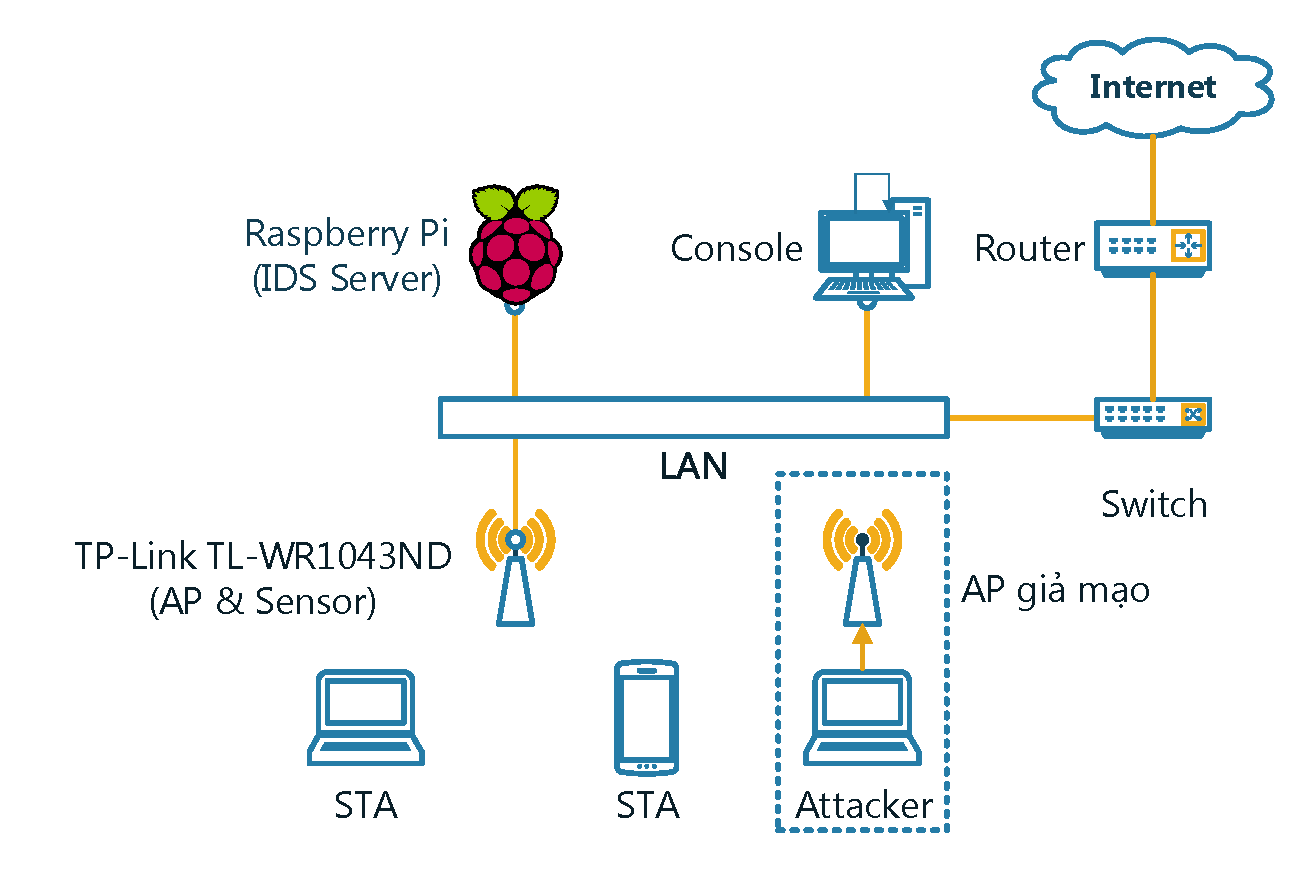
\includegraphics[width=0.9\textwidth]{diagram-wids-new-demo}
    \caption{
        \label{fig:diagram-wids-new-demo}
        Mô hình triển khai hệ thống KMA-WIDS}
\end{figure}

\item \emph{Switch:} một Switch thông thường, kết nối các thành phần của hệ thống WIDS, và kết nối với mạng có dây.
\item \emph{Router:} định tuyến và cung cấp kết nối Internet cho mạng nội bộ.
\item \emph{STA và Attacker:} các máy tính tham gia vào mạng không dây, Attacker sẽ là bên thực hiện các cuộc tấn công. Các STA còn lại là nạn nhân.
\item \emph{Console:} máy tính của quản trị viên, được kết nối vào mạng có dây. Máy tính này sẽ truy cập vào giao diện web Snorby trên IDS Server để giám sát hệ thống và nhận các cảnh báo xâm nhập.
\end{itemize}

\section{Triển khai hệ thống}
\subsection{Xây dựng và cài đặt OpenWrt cho AP}
Sản phẩm TP-Link TL-WR1043ND được đồ án lựa chọn để cài đặt làm AP và Sensor cho hệ thống WIDS. Với dung lượng bộ nhớ flash 8 MB, bộ nhớ RAM 64 MB, việc tự xây dựng một firmware tích hợp sẵn các gói phần mềm Kismet Drone, Daemonlogger và OpenVPN là cần thiết, giúp sử dụng bộ nhớ của thiết bị hiệu quả hơn. Hơn nữa, do các tập tin cấu hình mặc định đã được chỉnh sửa những thay đổi cần thiết, nên firmware sau khi xây dựng là một firmware có tính đóng gói, chỉ cần cài đặt lên thiết bị là có thể sử dụng ngay được.

Để làm được việc này, đầu tiên cần thay thế firmware gốc của nhà sản xuất bằng một firmware OpenWrt được xây dựng sẵn, có thể tải về từ website của dự án OpenWrt~\cite{openwrt2017wiki}. Sau đó thực hiện cài đặt và cấu hình các gói phần mềm thủ công, kiểm tra khả năng chạy thử thành công. Cuối cùng, sao chép các tập tin cấu hình này ra khỏi thiết bị và thực hiện xây dựng lại một firmware tích hợp với các tập tin cấu hình này. Vì không phải phần mềm nào cũng có thể tự khởi chạy khi thiết bị khởi động, nên cần viết thêm một vài script phục vụ công việc này. Firmware mới được tích hợp được cài đặt lại lên thiết bị.

\subsection{Cài đặt các thành phần cho IDS Server}
Do máy tính nhúng Raspberry Pi ban đầu sử dụng một thẻ nhớ trắng, nên cần cài đặt hệ điều hành Raspbian lên. Sau đó, tiến hành cài đặt lần lượt các gói phần mềm OpenVPN, Kismet, Snort, các phần mềm chuyển đổi định dạng dữ liệu là Sagan và Barnyard2, phần mềm giám sát an ninh Snorby và gói phần mềm Apache, MySQL để tạo một HTTP Server và cơ sở dữ liệu phục vụ cho Snorby. Chi tiết phiên bản phần mềm, cũng như các tập luật được trình bày trong phần Phụ lục B.

\section{Kiểm thử hệ thống}
\subsection{Phương pháp và kịch bản}
Hệ thống KMA-WIDS sẽ được kiểm thử bằng hai phương pháp kiểm thử, đầu tiên đó là xác định hệ thống có làm việc được và thực hiện chức năng phát hiện xâm nhập hay không, phương pháp nữa đó là đo thời gian phản hồi của hệ thống trong quá trình phát hiện xâm nhập.

Kịch bản sử dụng đó là thực hiện một số tấn công điển hình từ bên ngoài mạng và từ trong mạng. Kiểm tra khả năng phát hiện tấn công và tạo ra các cảnh báo bằng giao diện web Snorby. Ngoài ra, Kismet và Snort cũng cho phép lưu lại các tập tin pcap, có thể dựa vào đó để tính toán thời gian phản hồi của hệ thống trước các cuộc tấn công.

\subsection{Kiểm thử chức năng}
Kiểm thử chức năng nhằm mục đích kiểm tra việc hệ thống WIDS có làm việc đúng với chức năng của các IDS nói chung. Hệ thống KMA-WIDS này được mong đợi có thể phát hiện các tấn công từ cả bên trong và bên ngoài mạng không dây, và tạo ra các cảnh báo gửi tới giao diện web Snorby. Một số tấn công điển hình sẽ thực hiện đó là:

\begin{itemize}
\item \emph{Tấn công giả mạo AP:} Tấn công này sẽ tạo ra một AP giả mạo với địa chỉ MAC giống như AP hợp pháp, nhằm mục đích lừa cho các STA kết nối vào AP giả mạo.
\item \emph{Tấn công làm lụt khung hủy bỏ xác thực:} Tấn công làm lụt bằng cách liên tục gửi các khung hủy bỏ xác thực tới địa chỉ quảng bá, với địa chỉ MAC nguồn là của AP, làm cho các STA đang kết nối với AP bị ngắt kết nối.
\item \emph{Tấn công quét cổng:} Tấn công quét cổng nhằm dò quét các cổng dịch vụ đang mở trên một STA, nhằm tìm kiếm thông tin về các dịch vụ đang chạy, phục vụ cho các cuộc tấn công khác.
\item \emph{Tấn công khai thác lỗ hỏng bảo mật:} Tấn công khai thác một lỗ hỏng bảo mật bằng cách gửi các payload khai thác lỗ hỏng bảo mật đến STA, từ đó có thể mở một kết nối backdoor và điều khiển máy tính nạn nhân.
\end{itemize}

\subsection{Đo thời gian phản hồi}
Thời gian phản hồi ở đây là thời gian mà hệ thống sử dụng để phát hiện các tấn công và tạo ra cảnh báo. Thời gian phản hồi này có thể được tính toán từ các giá trị khác nhau của thời gian hệ thống cần để phát hiện một tấn công khi nó gửi cảnh báo. Trong tính toán thời gian phản hồi sẽ sử dụng tấn công làm lụt khung hủy bỏ xác thực.

\section{Kết quả kiểm thử}
\subsection{Một số hình ảnh giao diện Snorby}

\begin{figure}[H]
    \centering
    \frame{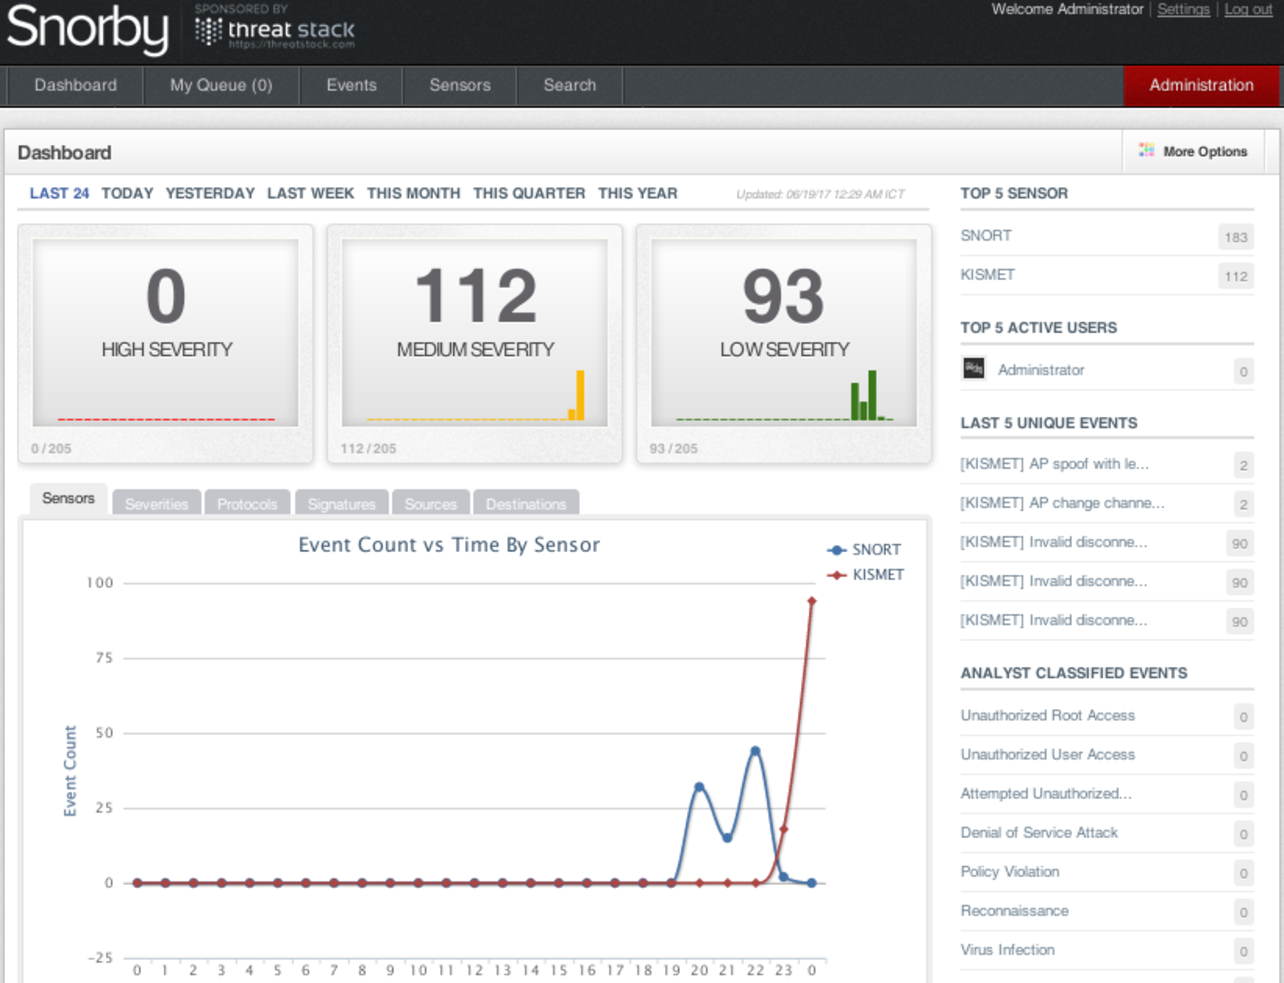
\includegraphics[width=0.95\textwidth]{snorby-dashboard}}
    \caption{
        \label{fig:snorby-dashboard}
        Giao diện bảng điều khiển của Snorby}
\end{figure}

Hình~\ref{fig:snorby-dashboard} là bảng điều khiển của Snorby, tại đây quản trị viên có thể thấy được tổng quan về số lượng sự kiện, mức độ nghiêm trọng, cũng có thể xuất báo cáo thành định dạng pdf.

Hình~\ref{fig:snorby-sensors} là danh sách các Sensor của hệ thống KMA-WIDS, bao gồm một Sensor nhận cảnh báo của Kismet và Sensor còn lại nhận cảnh báo từ Snort.

\begin{figure}[H]
    \centering
    \frame{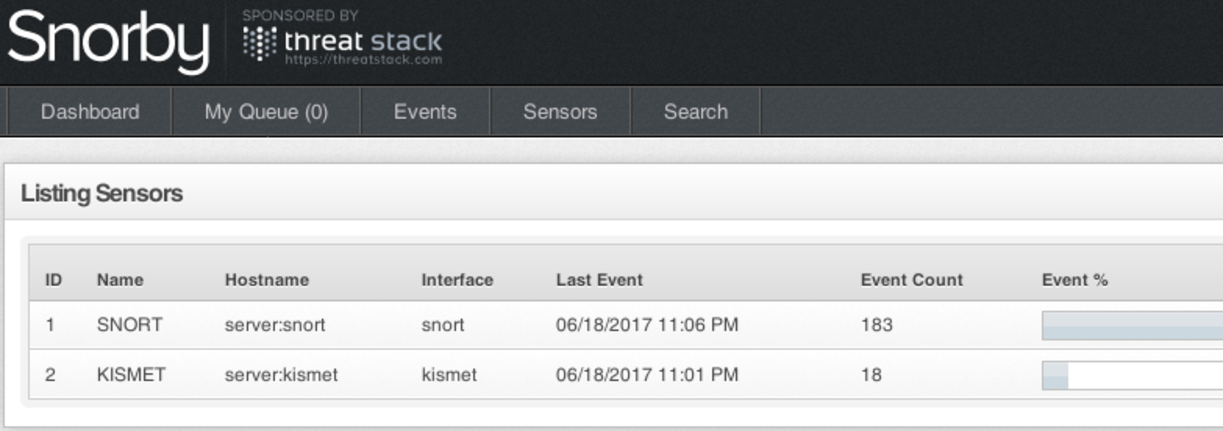
\includegraphics[width=1.0\textwidth]{snorby-sensors}}
    \caption{
        \label{fig:snorby-sensors}
        Danh sách các Sensor trên Snorby}
\end{figure}

Các Hình~\ref{fig:snorby-events} và Hình~\ref{fig:snorby-search} là giao diện quản lý sự kiện và giao diện tìm kiếm của Snorby.

\begin{figure}[H]
    \centering
    \frame{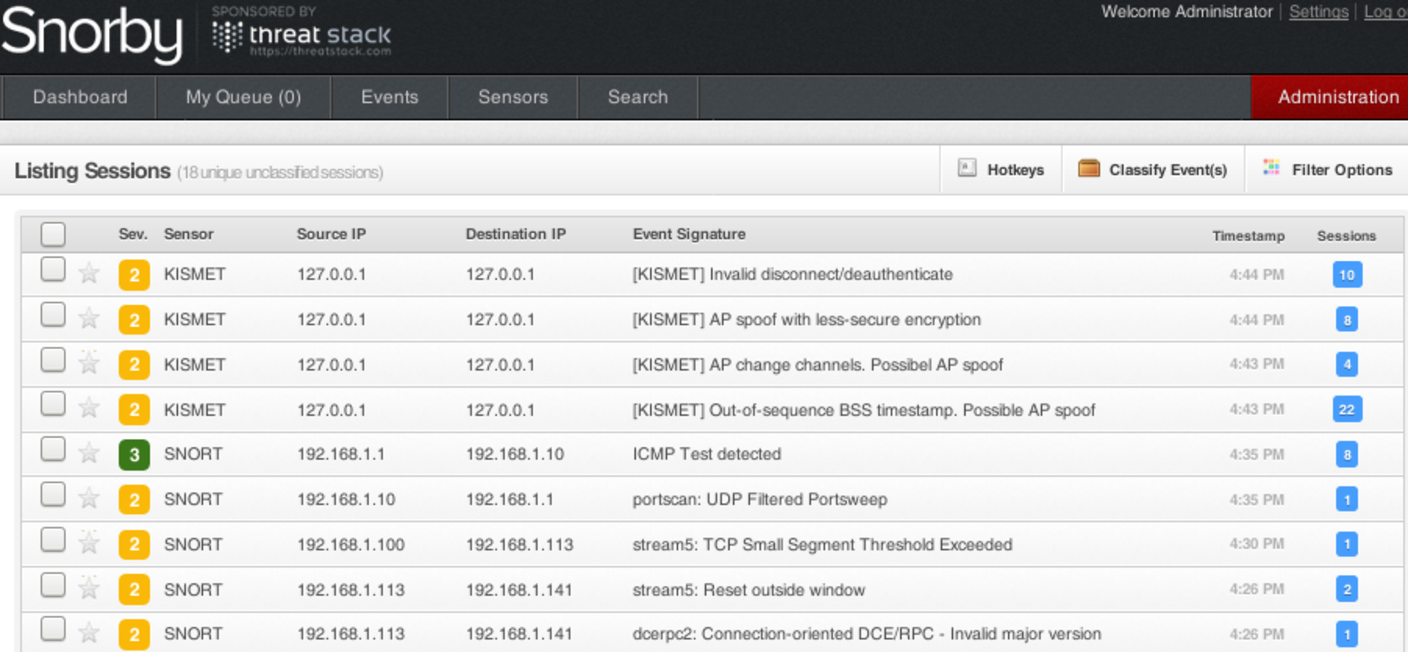
\includegraphics[width=1.0\textwidth]{snorby-events}}
    \caption{
        \label{fig:snorby-events}
        Giao diện quản lý sự kiện của Snorby}
\end{figure}

\begin{figure}[H]
    \centering
    \frame{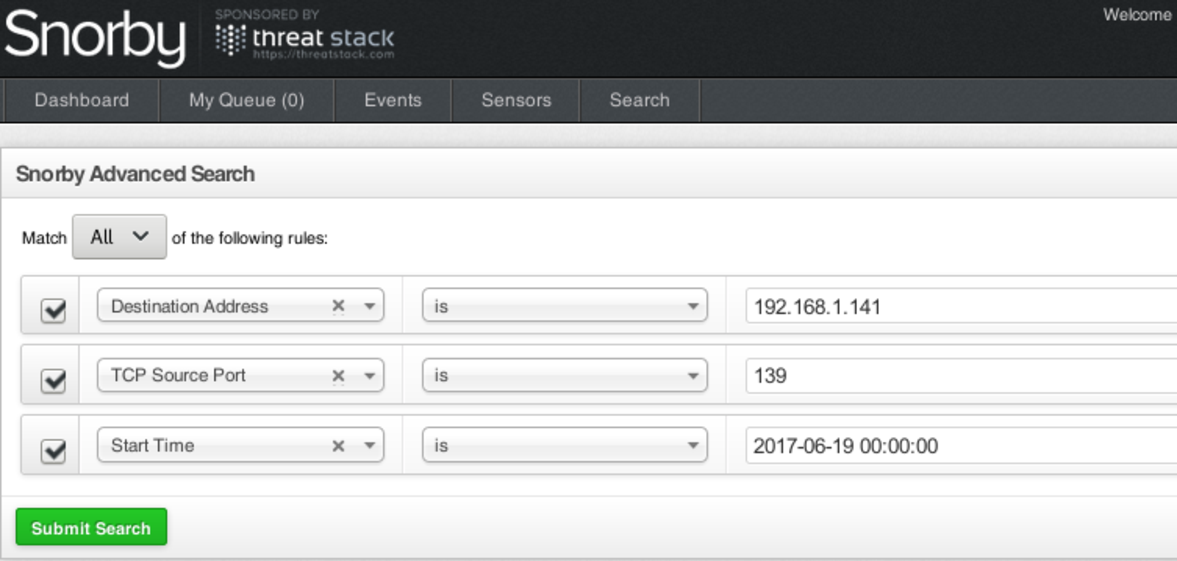
\includegraphics[width=1.0\textwidth]{snorby-search}}
    \caption{
        \label{fig:snorby-search}
        Chức năng tìm kiếm của Snorby}
\end{figure}

\subsection{Kiểm thử chức năng} \label{subsection:kiem-thu-chuc-nang}
\subsubsection*{a) Tấn công giả mạo AP}
Tấn công giả mạo AP sẽ được thực hiện bằng công cụ \emph{airbase-ng}. Công cụ này có thể chuyển đổi một máy tính với card mạng không dây thành một AP. Với một số thiết lập để trông giống AP hợp pháp, khi STA kết nối vào AP giả mạo, toàn bộ lưu lượng truy cập không dây sẽ bị kẻ tấn công chặn bắt và đọc được. Các bước tấn công có thể tóm tắt như sau:

\begin{itemize}
\item \emph{Bước 1:} Kiểm tra trạng thái các card mạng không dây đang hoạt động, chuyển card muốn sử dụng sang chế độ giám sát.
\item \emph{Bước 2:} Dùng công cụ airbase-ng để tạo AP giả mạo với địa chỉ MAC, ESSID và số hiệu kênh giống với AP hợp pháp.
\item \emph{Bước 3:} Cấu hình địa chỉ IP cho giao diện mạng làm AP mà airbase-ng tạo ra.
\item \emph{Bước 4:} Thiết lập định tuyến, NAT để cung cấp kết nối Internet cho AP giả mạo.
\item \emph{Bước 5:} Thiết lập và chạy dịch vụ DHCP để tự động cấp phát khi một STA tham gia vào mạng của AP giả mạo.
\item \emph{Bước 6:} Bật tính năng chuyển tiếp gói tin IP.
\item \emph{Bước 7:} Sử dụng một công cụ phân tích mạng để chặn bắt gói tin, ví dụ tcpdump.
\end{itemize}

Kismet có thể phát hiện được các tấn công giả mạo AP. Cụ thể, Kismet phát hiện tấn công này bằng cách phân tích các nhãn thời gian (timestamp) của các khung báo hiệu được gửi từ AP mà nó giám sát. Các nhãn thời gian có chức năng là để đồng bộ giao dịch giữa STA và AP, có giá trị rất nhỏ và liên tục, do vậy rất khó bị giả mạo. Cảnh báo BSSTIMESTAMP~\cite{mike2016kismet} của Kismet mô tả một nhãn thời gian có số thứ tự không hợp lệ hoặc ngoài phạm vi cho phép có thể cho thấy một tấn công giả mạo AP.

Hình~\ref{fig:bss-timestamp-snorby} là hình ảnh của cảnh báo BSSTIMESTAMP trên giao diện Snorby.

\begin{figure}[H]
    \centering
    \frame{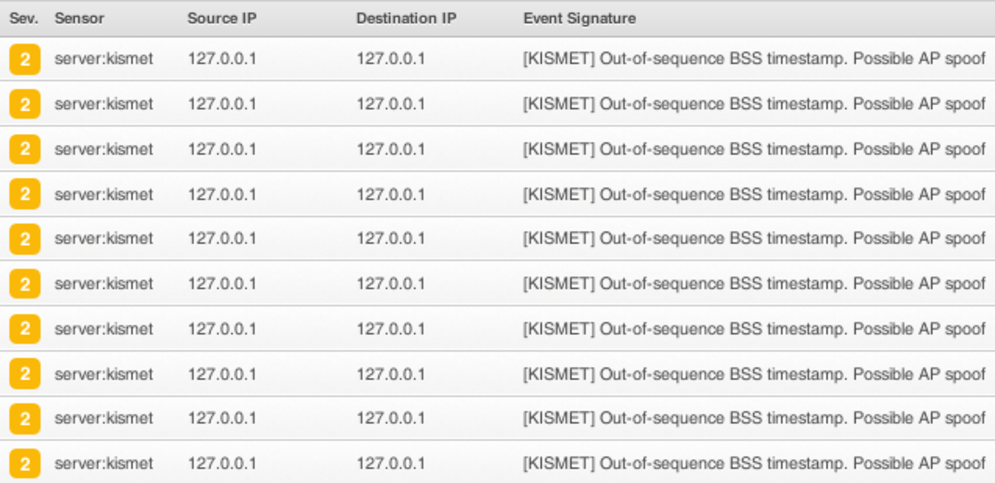
\includegraphics[width=1.0\textwidth]{bss-timestamp-snorby}}
    \caption{
        \label{fig:bss-timestamp-snorby}
        Cảnh báo BSSTIMESTAMP trên Snorby}
\end{figure}

Kismet cũng lưu lại các khung thu thập được vào tập tin định dạng \emph{pcap}, có thể đọc được bằng phần mềm Wireshark. Hình~\ref{fig:bss-timestamp-wireshark} là hình ảnh các khung được đọc bằng phần mềm Wireshark, cho thấy giá trị trường \emph{Timestamp} có thể đọc được dễ dàng.

\begin{figure}[H]
    \centering
    \frame{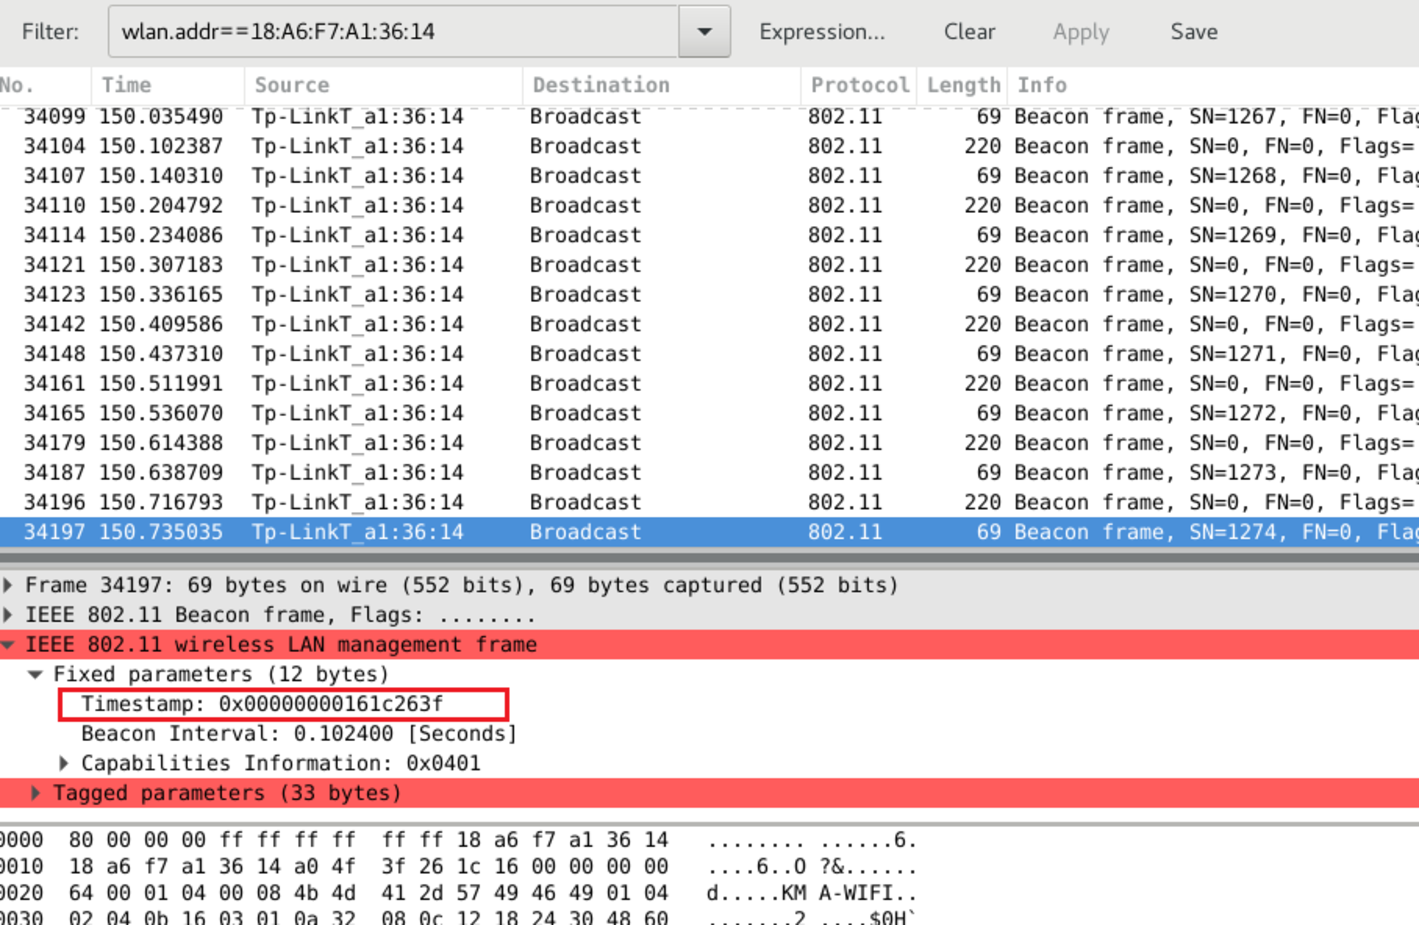
\includegraphics[width=1.0\textwidth]{bss-timestamp-wireshark}}
    \caption{
        \label{fig:bss-timestamp-wireshark}
        Các khung được đọc bằng phần mềm Wireshark}
\end{figure}

\subsubsection*{b) Tấn công làm lụt khung hủy bỏ xác thực}
Công cụ được sử dụng trong tấn công này là \emph{aircrack-ng}. Aircrack-ng là một công cụ đa tính năng, thường được sử dụng để đánh giá hệ thống mạng không dây, ví dụ như tấn công dò khóa WEP, WPA-PSK, tấn công làm lụt khung xác thực và khung hủy bỏ xác thực, thậm chí tấn công tiêm các gói ARP. Trong kiểm thử này sẽ sử dụng tấn công làm lụt bằng các khung hủy bỏ xác thực để ngắt kết nối của tất cả các STA đến AP.  Tấn công này thường được sử dụng để mở đầu một tấn công Man-in-the-middle, nhằm ngắt kết nối các STA với AP hợp pháp làm cho chúng kết nối tới AP giả mạo.

Các câu lệnh đã được sử dụng để tấn công:\\

\begin{lstlisting}
# airmon-ng start wlp3s0
# airodump-ng wlp3s0mon
# aireplay-ng -0 1 -a 18:A6:F7:A1:36:14 -c FF:FF:FF:FF:FF:FF wlp3s0mon
\end{lstlisting}

Trong đó, câu lệnh đầu dùng để bật chế độ giám sát cho giao diện mạng không dây. Tiếp theo là hiển thị các AP trong phạm vi, từ đó xác định được địa chỉ MAC của AP cần tấn công. Cuối cùng là thực hiện gửi các khung hủy bỏ xác thực đến địa chỉ quảng bá.

\begin{figure}[H]
    \centering
    \frame{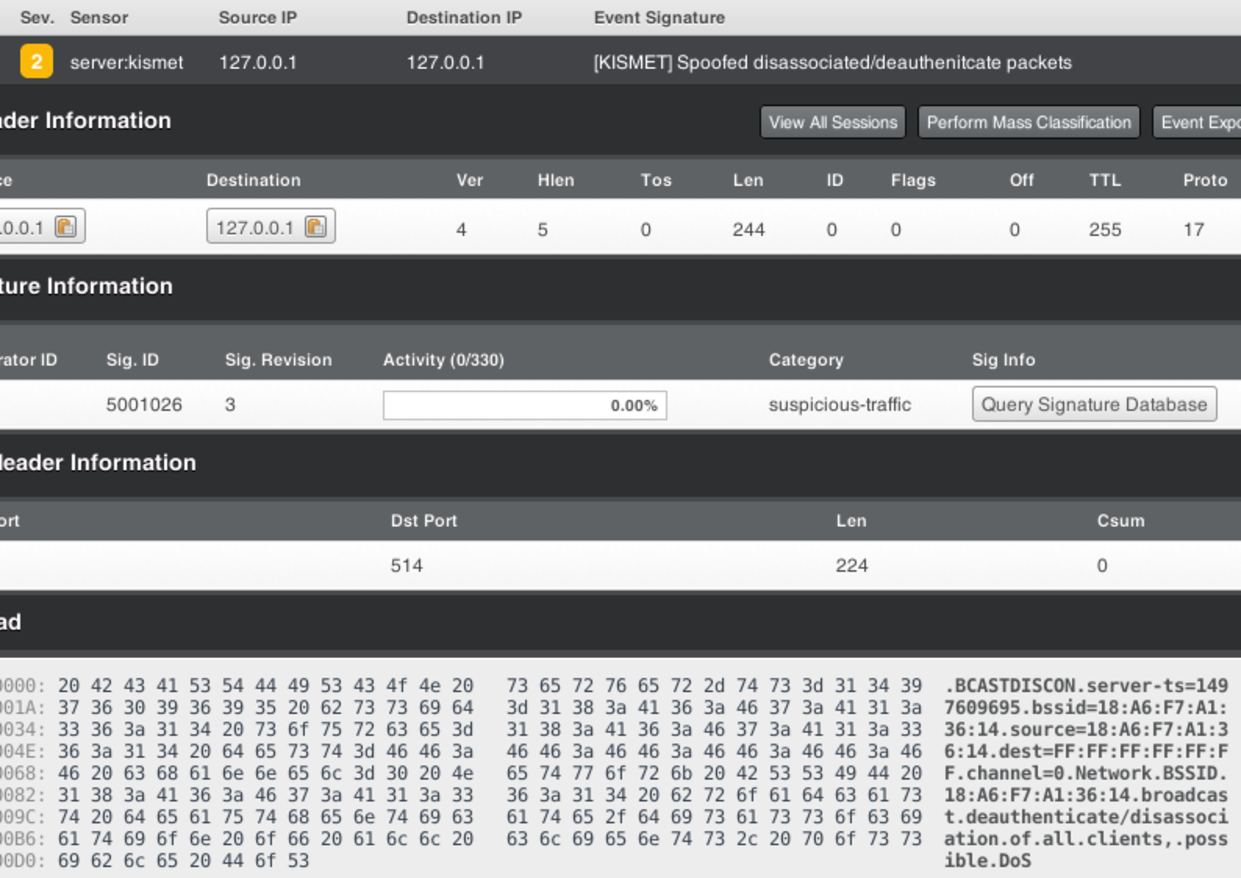
\includegraphics[width=1.0\textwidth]{deauth-snorby}}
    \caption{
        \label{fig:deauth-snorby}
        Chi tiết cảnh báo tấn công làm lụt khung hủy bỏ xác thực}
\end{figure}

Theo tài liệu Kismet~\cite{mike2016kismet}, Kismet hoàn toàn phát hiện được tấn công dạng này. Kết quả kiểm thử cũng cho thấy điều đó. Hình~\ref{fig:deauth-snorby} là chi tiết một cảnh báo tấn công làm lụt khung hủy bỏ xác thực trên Snorby. Ngoài ra, tập tin được Kismet lưu lại cũng dễ dàng quan sát được các khung hủy bỏ xác thực, cụ thể như Hình~\ref{fig:deauth-wireshark}. Trong hình có sử dụng câu lệnh lọc "\emph{wlan.addr==18:A6:F7:A1 :36:14 \&\& wlan.fc.type\_subtype==0x0c}", vế đầu là địa chỉ MAC của AP, vế sau là loại khung, \emph{0x0c} là mã khung phụ của khung quản lý, chính là khung hủy bỏ xác thực đang được xét.

\begin{figure}[H]
    \centering
    \frame{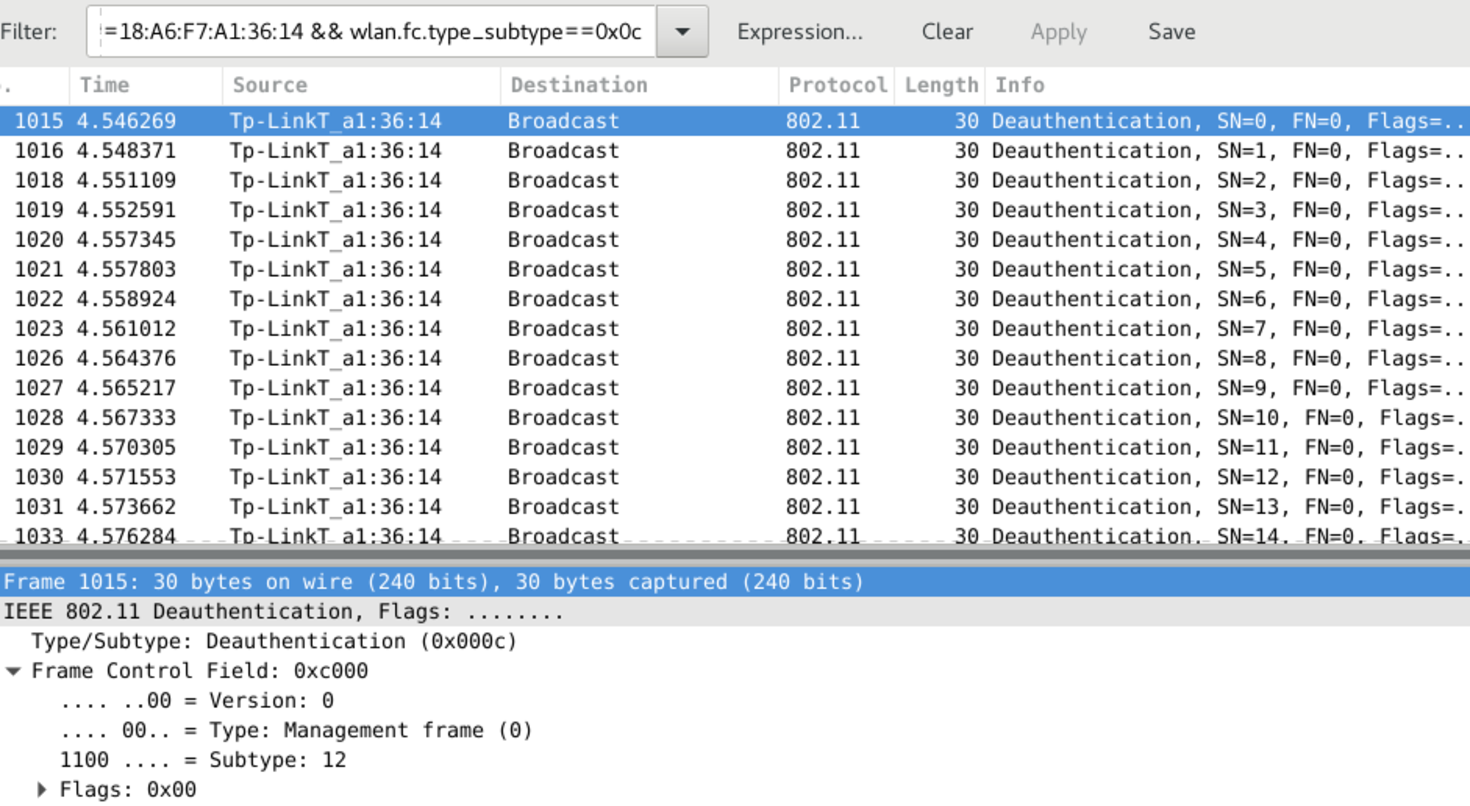
\includegraphics[width=1.0\textwidth]{deauth-wireshark}}
    \caption{
        \label{fig:deauth-wireshark}
        Hình ảnh các khung hủy bỏ xác thực trong Wireshark}
\end{figure}

\subsubsection*{c) Tấn công quét cổng}
Kiểm thử này sử dụng một công cụ quét mạng nổi tiếng, đó là \emph{nmap}. Dưới đây là kết quả của việc quét một máy tính Windows XP, đang tham gia vào mạng không dây. Câu lệnh nmap có ý nghĩa là kiểu quét TCP SYN, quét các cổng từ 1 đến 65535, tùy chọn phát hiện phiên bản của hệ điều hành và dịch vụ được bật. Kiểu quét TCP SYN không thực hiện quá trình bắt tay ba bước hoàn chỉnh, nó chỉ gửi đi gói SYN, sau đó chờ phản hồi. Nếu phản hồi có cờ SYN/ACK được bật, tức là cổng đó đang mở, cờ RST tức là cổng đó đang đóng. Nếu không có phản hồi gì sau một vài lần gửi, hoặc phản hồi chứa mã lỗi ICMP unreachable, cho thấy cổng đó đã được bảo vệ bởi tường lửa~\cite{lyon2009nmap}.\\

\begin{lstlisting}
# nmap -p1-65535 -sV -sS -O 192.168.1.141
Starting Nmap 7.40 ( https://nmap.org ) at 2017-06-19 01:16 +07
Nmap scan report for client.lan (192.168.1.141)
Host is up (0.00031s latency).
Not shown: 65532 closed ports
PORT    STATE SERVICE      VERSION
\end{lstlisting}


\begin{lstlisting}
135/tcp open  msrpc        Microsoft Windows RPC
139/tcp open  netbios-ssn  Microsoft Windows netbios-ssn
445/tcp open  microsoft-ds Microsoft Windows XP microsoft-ds

Device type: general purpose
Running: Microsoft Windows XP
OS CPE: cpe:/o:microsoft:windows_xp::sp2 cpe:/o:microsoft:windows_xp::sp3
OS details: Microsoft Windows XP SP2 or SP3
Network Distance: 1 hop
Service Info: OSs: Windows, Windows XP; CPE: cpe:/o:microsoft:windows, cpe:/o:microsoft:windows_xp
\end{lstlisting}

\begin{figure}[H]
    \centering
    \frame{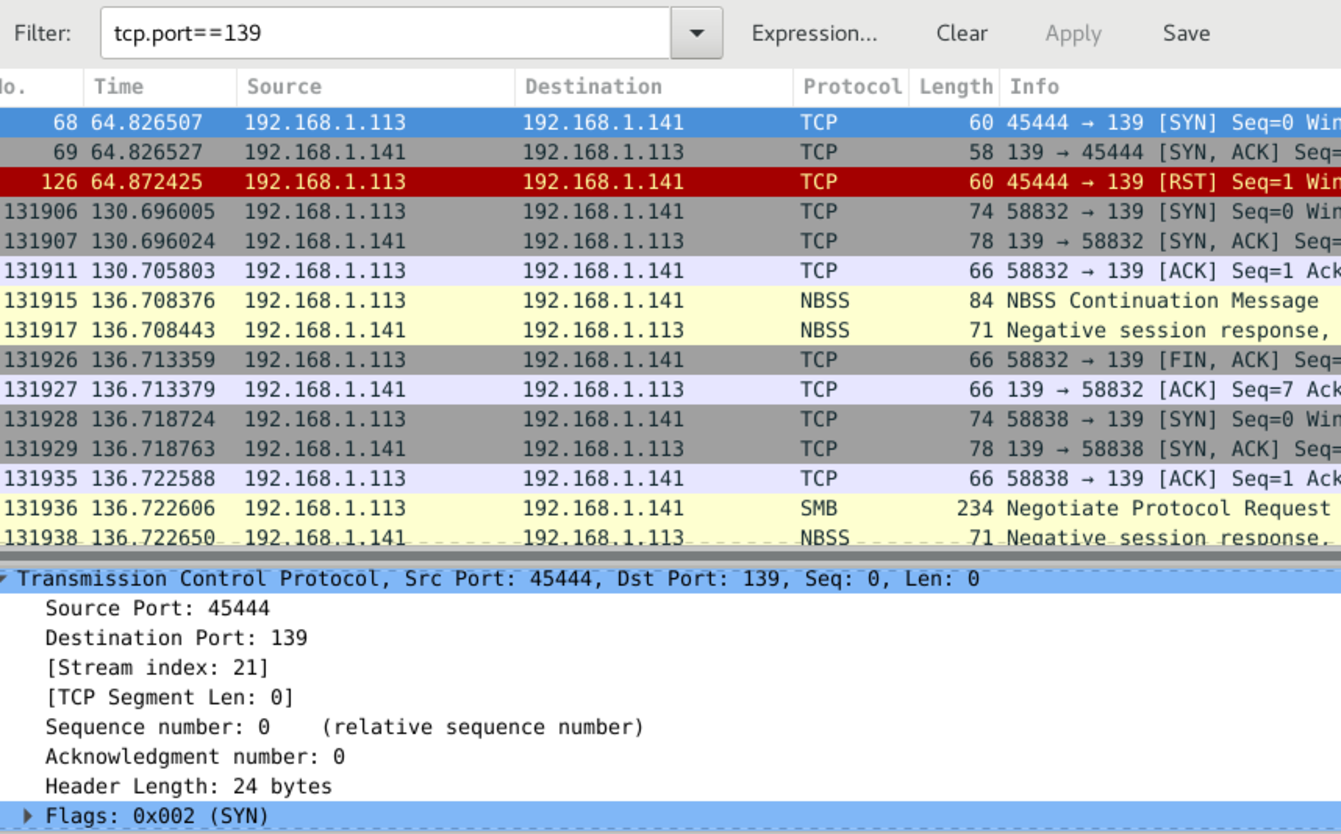
\includegraphics[width=1.0\textwidth]{port-scanning-139}}
    \caption{
        \label{fig:port-scanning-139}
        Các gói tin quét cổng thu thập được}
\end{figure}

Hình~\ref{fig:port-scanning-139} là gói tin pcap được thu thập ở máy nạn nhân. Trong đó, \emph{192.168.1.113} là địa chỉ IP của máy tấn công, \emph{192.168.1.141} là địa chỉ IP của máy nạn nhân. Câu lệnh lọc "\emph{tcp.port==139}" được sử dụng nhằm lọc các gói tin có liên quan đến cổng 139, chính là số hiệu cổng đang mở trên máy nạn nhân. Có thể thấy ngay qua 3 gói tin đầu tiên, trước hết kẻ tấn công mở kết nối TCP đến máy nạn nhân qua cổng 139 bằng gói tin có cờ SYN bật; tiếp đến, máy nạn nhân gửi lại gói tin có cờ SYN/ACK được bật, do đó kẻ tấn công biết được cổng 139 đang mở. Nếu như một quá trình bắt tay ba bước bình thường, máy tấn công sẽ gửi lại gói tin có cờ ACK được bật để thiết lập kết nối, tuy nhiên, nó đã gửi lại gói RST. Xét tiếp các gói tin phía sau, do kẻ tấn công muốn biết rõ dịch vụ đang chạy qua cổng 139 là dịch vụ gì, nên nó đã thiết lập quá trình bắt tay ba bước đầy đủ, để kết nối với máy nạn nhân, quá đó biết được dịch vụ cụ thể là gì.

Tấn công này được phát hiện bằng Snort. Cảnh báo được gửi tới Snorby như Hình~\ref{fig:port-scanning-attack-snorby}.

\begin{figure}[H]
    \centering
    \frame{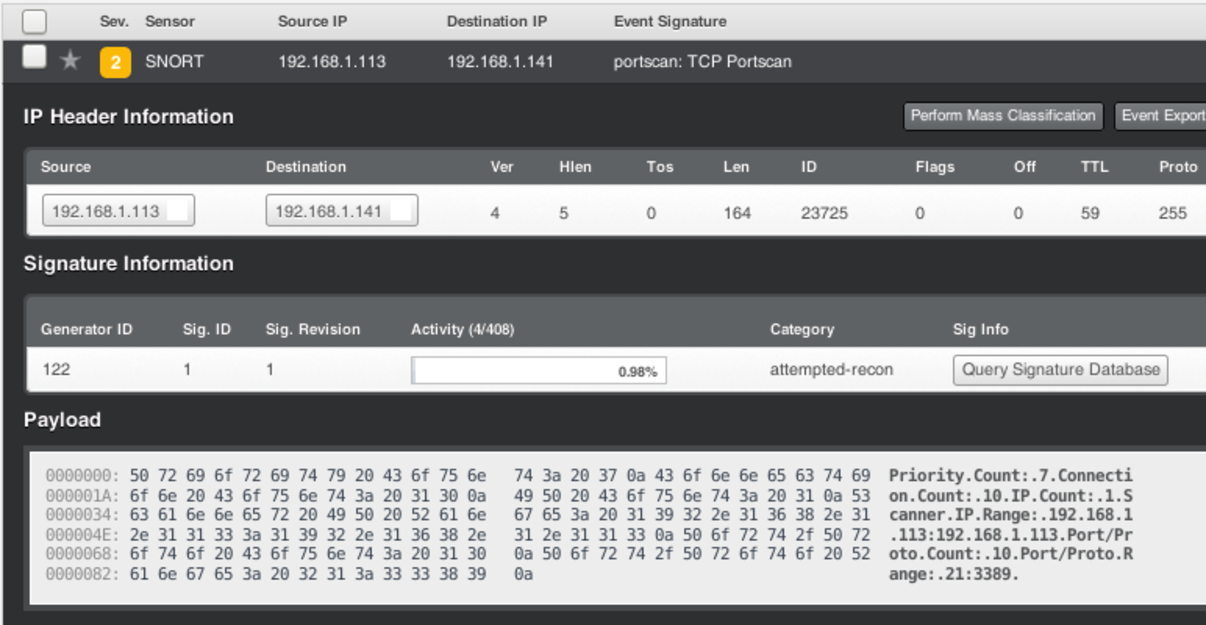
\includegraphics[width=1.0\textwidth]{port-scanning-attack-snorby}}
    \caption{
        \label{fig:port-scanning-attack-snorby}
        Cảnh báo tấn công quét cổng trên Snorby}
\end{figure}

\subsubsection*{d) Khai thác lỗ hỏng bảo mật MS08-067}
MS08-067 là một lỗ hỏng điển hình trên hệ điều hành Windows, cho phép kẻ tấn công thực thi mã lệnh từ xa. Cụ thể, giao thức RPC của dịch vụ Server Service trong Windows hỗ trợ một thủ tục được gọi từ xa và xử lý các yêu cầu đổi đường dẫn (ví dụ, \emph{{\textbackslash \textbackslash}C{\textbackslash}Program Files{\textbackslash}..{\textbackslash}Windows}) về định dạng đường dẫn Canonicalization ngắn gọn hơn (\emph{{\textbackslash \textbackslash}C{\textbackslash}Windows}). Tuy nhiên, với một đường dẫn quá dài, Windows xử lý không tốt dẫn đến lỗ hỏng tràn bộ đệm~\cite{microsoft2008ms08067}. Bằng cách chuyển hướng lỗ hỏng tràn bộ đệm, kẻ tấn công có thể tiêm vào các mã lệnh và thực thi từ xa theo ý mình.

Tấn công này được thực hiện sử dụng công cụ Metasploit, tóm tắt các câu lệnh tấn công như sau:\\

\begin{lstlisting}
msf > use exploit/windows/smb/ms08_067_netapi
msf exploit(ms08_067_netapi) > show targets
            ...targets...
msf exploit(ms08_067_netapi) > set TARGET <target-id>
msf exploit(ms08_067_netapi) > show options
            ...show...
msf exploit(ms08_067_netapi) > set RHOST <ip-address>
msf exploit(ms08_067_netapi) > exploit
\end{lstlisting}

\begin{figure}[H]
    \centering
    \frame{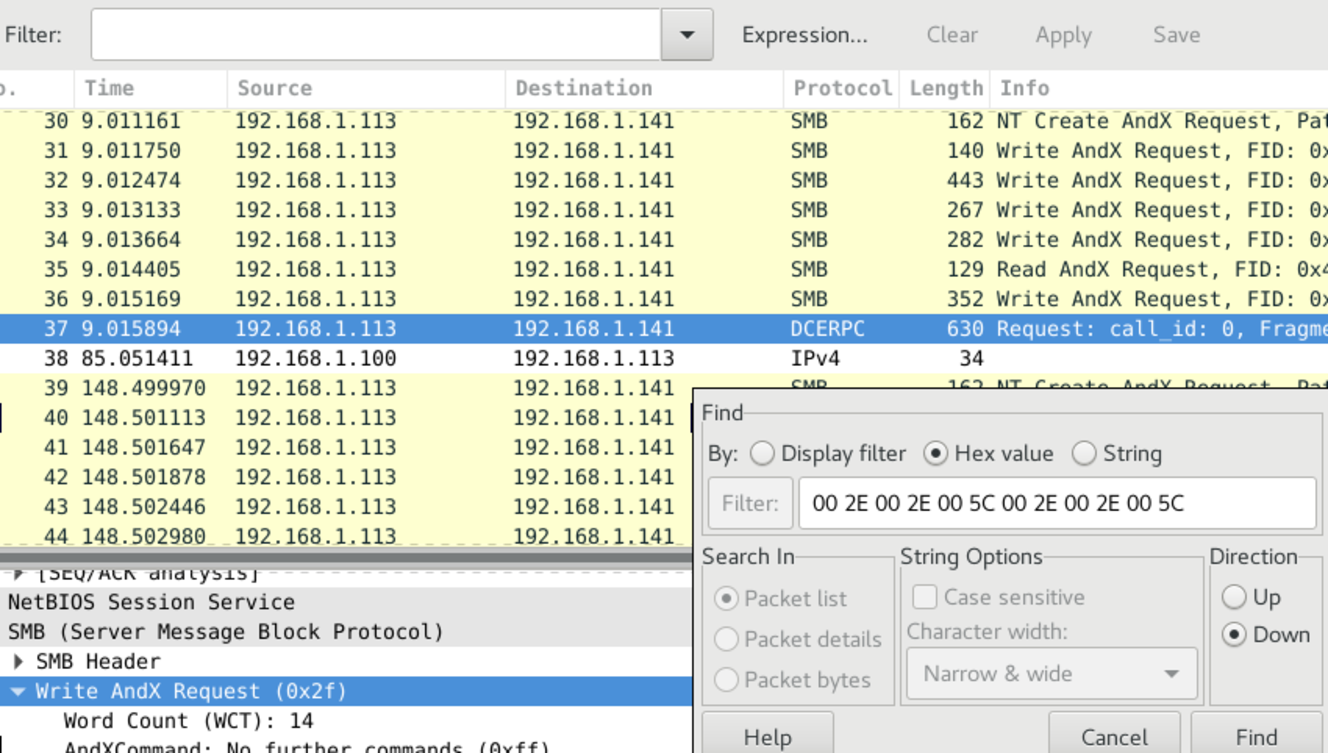
\includegraphics[width=1.0\textwidth]{ms08-067-snort-wireshark}}
    \caption{
        \label{fig:ms08-067-snort-wireshark}
        Các gói tin từ tấn công khai thác lỗ hỏng MS08-067}
\end{figure}

Hình~\ref{fig:ms08-067-snort-wireshark} là hình ảnh các gói tin mà Snort lưu lại. Trong phần tìm kiếm là các byte lấy từ luật mà Snort dùng để phát hiện tấn công này, hoàn toàn khớp với dữ liệu thu thập được. Với việc cấu hình luật phù hợp, Snort có thể phát hiện tấn công này và đưa ra cảnh báo tới giao diện Snorby như Hình~\ref{fig:ms08-067-snort-snorby}. Tấn công này được phân loại mức nghiêm trọng là 1, cao nhất trong ba mức nghiêm trọng của Snorby.

\begin{figure}[H]
    \centering
    \frame{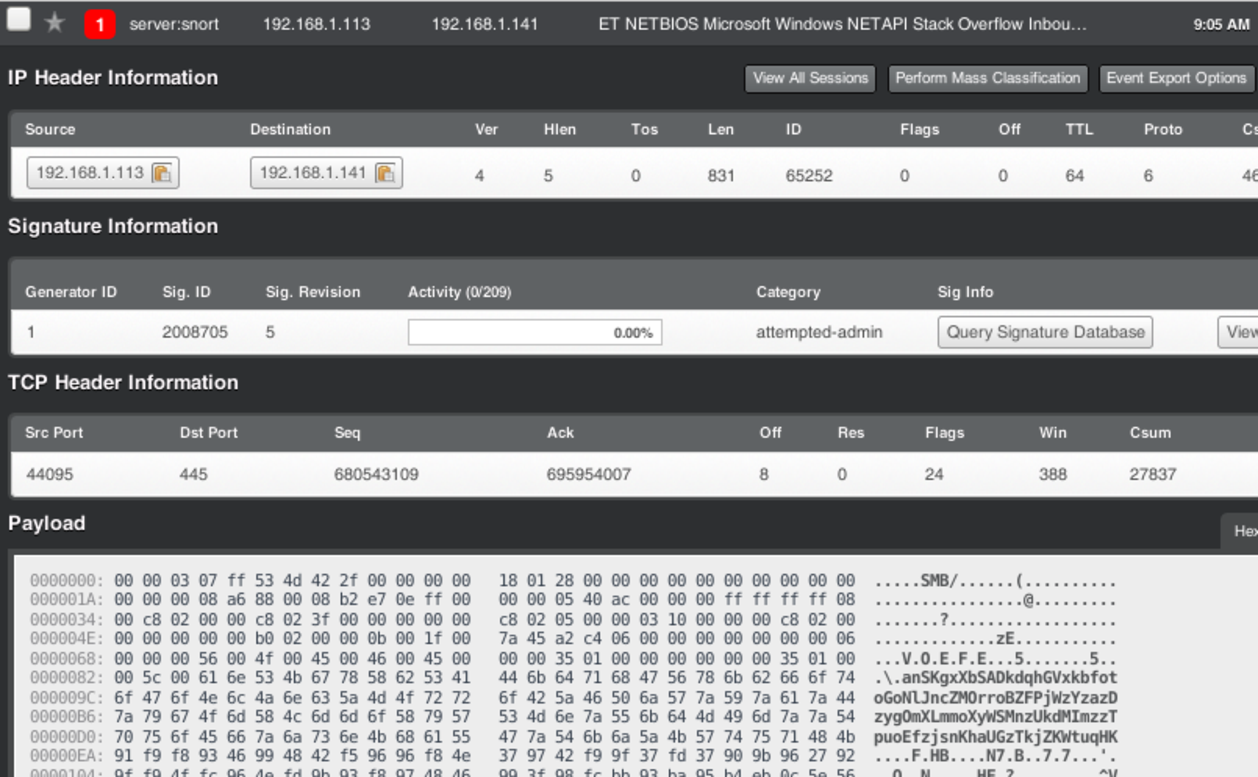
\includegraphics[width=1.0\textwidth]{ms08-067-snort-snorby}}
    \caption{
        \label{fig:ms08-067-snort-snorby}
        Cảnh báo tấn công khai thác lỗ hỏng MS08-067 trên Snorby}
\end{figure}

\subsection{Đo thời gian phản hồi}
Để đo thời gian phản hồi, đồ án tập trung vào tấn công làm lụt khung hủy bỏ xác thực. Tấn công này gửi liên tục nhiều khung hủy bỏ xác thực, do đó có thể đo được thời gian, số lượng khung, cũng như số lượng cảnh báo. Số liệu phân tích được lấy từ tập tin pcap trong phần kiểm thử chức năng.

Thời gian phản hồi được tính toán từ các thời gian khác nhau từ khi tấn công gửi đi khung hủy bỏ xác thực cho đến khi tấn công được phát hiện bởi Kismet. Các trường giá trị thời gian trong tập tin pcap có thể đọc được bằng phần mềm Wireshark như Hình~\ref{fig:deauth-attack-detect}.

\begin{figure}[H]
    \centering
    \frame{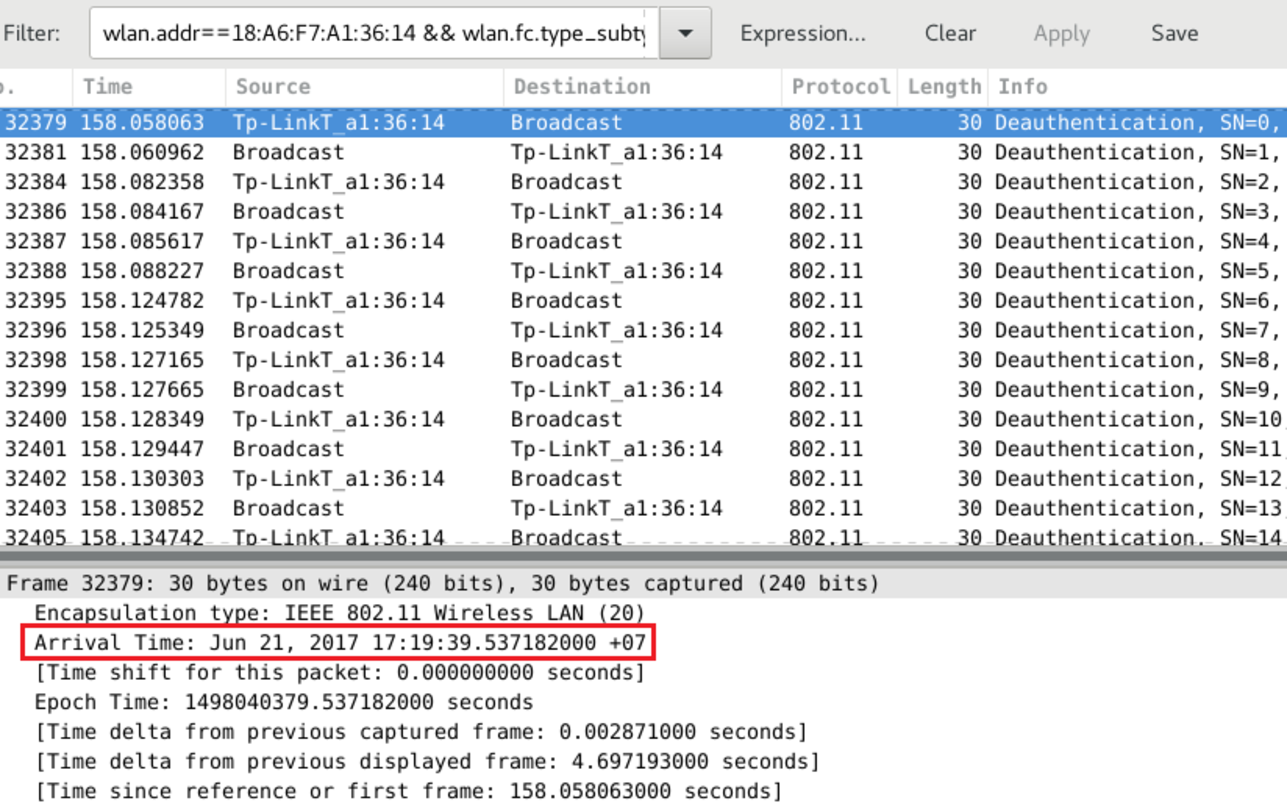
\includegraphics[width=1.0\textwidth]{deauth-attack-detect}}
    \caption{
        \label{fig:deauth-attack-detect}
        Thời gian bắt đầu phát hiện khung đầu tiên}
\end{figure}

Hình trên cho thấy, Kismet phát hiện khung hủy bỏ xác thực đầu tiên nhận được từ kẻ tấn công có \emph{Sequence Number (SN) = 0} vào thời gian \emph{Jun 21, 2017 17:19:39.537182000 +07}. Mỗi khung có một Sequence Number duy nhất, giá trị này sẽ được tăng lên khi một STA gửi cùng một khung giống với khung trước đó. Giá trị lớn nhất của SN là 4096. Sau khi đạt giá trị lớn nhất, số SN sẽ bắt đầu lại từ 0~\cite{guo2005sequence}.

Để đo được thời gian phản hồi của hệ thống WIDS, về phía kẻ tấn công cũng đã chạy Kismet để tự thu thập lại các khung nhằm xác định thời gian gửi đi. Hình~\ref{fig:deauth-attack-detect} là thông tin thời gian gửi của khung đầu tiên mà máy tấn công thu thập được.

Kẻ tấn công gửi khung hủy bỏ xác thực đầu tiên \emph{SN = 0} vào thời gian \emph{Jun 21, 2017 17:19:39.534660000 +07}. Sự khác nhau về thời gian từ khi khung tấn công được gửi tới khi Kismet của hệ thống WIDS phát hiện được là chậm hơn \emph{0.002522000} giây. Bảng~\ref{tab:response-time-table} là số liệu thống kê trong 10 khung đầu tiên.

\begin{figure}[H]
    \centering
    \frame{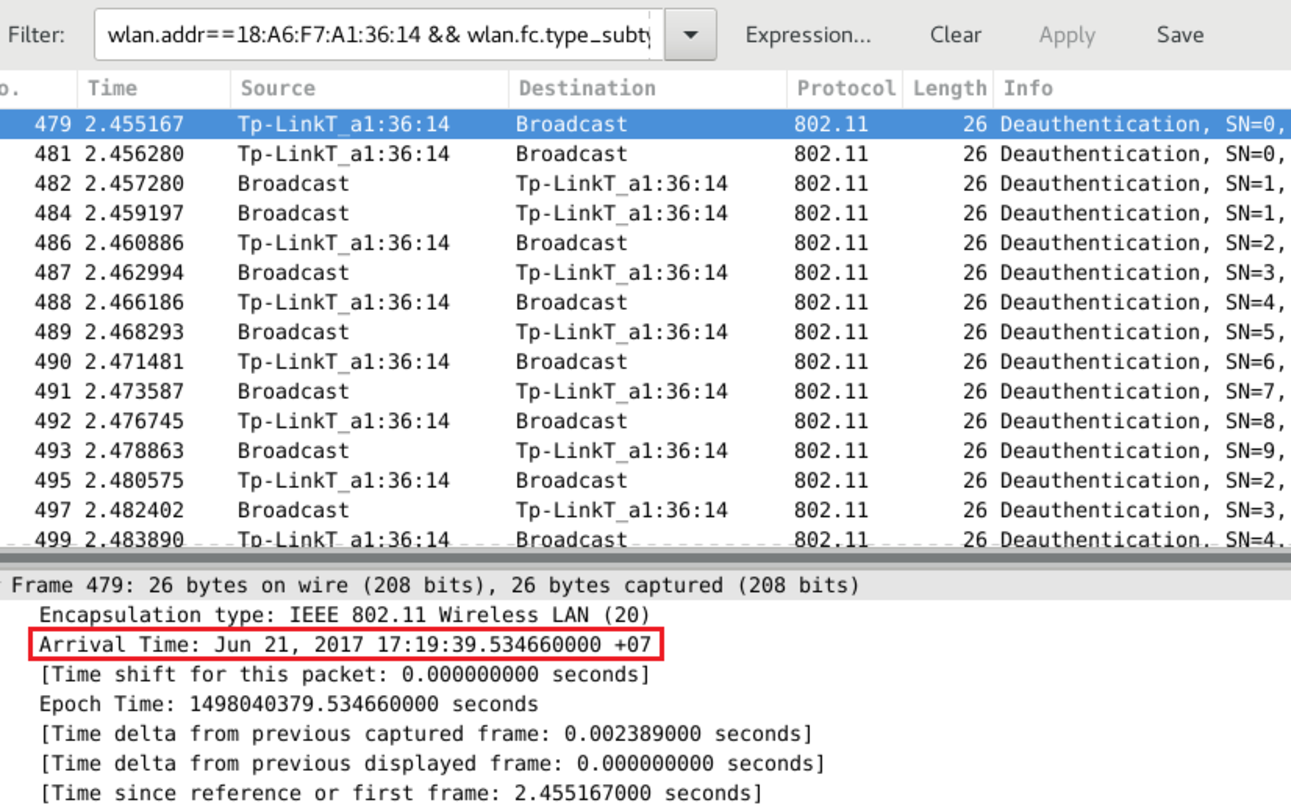
\includegraphics[width=1.0\textwidth]{deauth-attack-sent}}
    \caption{
        \label{fig:deauth-attack-sent}
        Thời gian bắt đầu gửi khung đầu tiên}
\end{figure}

\begin{table}[H]
\centering
\small
\setlength{\extrarowheight}{1pt}
\caption{\label{tab:response-time-table}Thống kê thời gian phản hồi trong 10 khung đầu tiên}
\begin{tabular}{|c|c|c|c|}
\hline
\textbf{SN} & \textbf{Thời gian gửi} & \textbf{Kismet phát hiện} & \textbf{Thời gian phản hồi} \\ \hline
0           & 17:19:39.534660000     & 17:19:39.537182000        & 0.002522000                 \\ \hline
1           & 17:19:39.536773000     & 17:19:39.540081000        & 0.003308000                 \\ \hline
2           & 17:19:39.540379000     & 17:19:39.561477000        & 0.021098000                 \\ \hline
3           & 17:19:39.542487000     & 17:19:39.563286000        & 0.020799000                 \\ \hline
4           & 17:19:39.545679000     & 17:19:39.564736000        & 0.019057000                 \\ \hline
5           & 17:19:39.547786000     & 17:19:39.567346000        & 0.019560000                 \\ \hline
6           & 17:19:39.550974000     & 17:19:39.603901000        & 0.052927000                 \\ \hline
7           & 17:19:39.553080000     & 17:19:39.604468000        & 0.051388000                 \\ \hline
8           & 17:19:39.556238000     & 17:19:39.606284000        & 0.050046000                 \\ \hline
9           & 17:19:39.558356000     & 17:19:39.606784000        & 0.048428000                 \\ \hline
\multicolumn{3}{|c|}{\textbf{Trung bình}}                        & \textbf{0.028913300}        \\ \hline
\end{tabular}
\end{table}

Vậy thời gian phản hồi trung bình cho các tấn công đầu tiên là \emph{0.028913300} giây. Với việc kiểm thử thời gian phản hồi, cho thấy hệ thống KMA-WIDS có khả năng phản hồi gần như lập tức trước các tấn công. Tuy nhiên, do thiết bị AP cũng đồng thời là WIDS Sensor, nên tấn công làm lụt khung hủy bỏ xác thực đang trực tiếp tấn công lên WIDS Sensor, dẫn đến thời gian phản hồi có xu hướng tăng theo thời gian, tức là hiệu suất của WIDS Sensor bị giảm.

\section{Tổng kết và đánh giá hệ thống}
Như vậy, qua bốn chương đã trình bày, đồ án đã nghiên cứu và triển khai thành công hệ thống KMA-WIDS với các chức năng chính: giám sát và phát hiện các tấn công từ bên trong và bên ngoài mạng WiFi, đưa ra các cảnh báo kịp thời thông qua giao diện quản trị. Khả năng phát hiện các tấn công bên ngoài mạng của hệ thống không kém gì so với một giải pháp dành cho doanh nghiệp.

Về các tấn công bên trong mạng WiFi, chúng cũng đa dạng và tương tự như các tấn công bên trong mạng có dây. Đồ án chỉ kiểm thử khả năng phát hiện một số tấn công điển hình, cấu hình luật phù hợp để Snort có thể phát hiện và tạo ra các cảnh báo. Qua đó thấy được, hệ thống WIDS đề xuất hoàn toàn có khả năng phát hiện các tấn công bên trong mạng WiFi.

Sau đây là tóm tắt các ưu điểm nổi bật của hệ thống KMA-WIDS:

\begin{itemize}
\item Hệ thống KMA-WIDS được tích hợp lên thiết bị Access Point thông thường, và máy tính nhúng Raspberry Pi, mang lại sự phù hợp về hiệu quả và chi phí.
\item Hệ thống có khả năng phát hiện được cả tấn công từ bên trong và bên ngoài mạng WiFi, bảo vệ hạ tầng mạng WiFi và người dùng khỏi các mối đe dọa bảo mật.
\item Hệ thống cũng cung cấp giao diện quản trị Snorby trực quan và dễ sử dụng.
\item Bằng việc ứng dụng các phần mềm mã nguồn mở, hệ thống có khả năng mở rộng cao, các phần mềm mã nguồn mở này vẫn đang được cộng đồng phát triển từng ngày.
\item Hệ thống sử dụng các bản phân phối dựa trên Linux, nên có thể tương thích với hầu hết các loại phần cứng phổ biến.\\
\end{itemize}

Bên cạnh đó, vì thời gian nghiên cứu còn hạn chế, hệ thống KMA-WIDS vẫn còn tồn tại một số vấn đề cần quan tâm như:

\begin{itemize}
\item Hệ thống hiện chỉ hỗ trợ phát hiện các tấn công, chưa có biện pháp để ngăn chặn các tấn công khi chúng xảy ra.
\item Khả năng phát hiện tấn công bên ngoài phụ thuộc hoàn toàn vào Kismet, không hỗ trợ viết luật để nhận diện tấn công mới. Snort cần được cấu hình tập luật phù hợp, để có thể phát hiện các tấn công bên trong mạng.
\item Hiệu năng của hệ thống cần được tối ưu hơn nữa để có thể triển khai rộng rãi trong thực tế. Công việc này đòi hỏi quá trình nghiên cứu và phát triển để làm cho các phần mềm thực sự hoạt động hiệu quả trên thiết bị nhúng.\\
\end{itemize}

Những vấn đề này sẽ được đề cập rõ hơn trong phần~\ref{section:huong-phat-trien} - Hướng phát triển của hệ thống trong chương tiếp theo.

